% TODO:
% * List the feature functions that we use in our decoder.

\documentclass[11pt]{article}
%\usepackage{acl08}
\usepackage{acl-ijcnlp2009}
\usepackage{times}
\usepackage{latexsym}
\usepackage{multirow}
%\usepackage{clrscode}
\usepackage{amscd}
\usepackage{amsmath}
\usepackage{amssymb}
\usepackage{color}
\usepackage{epsfig}
\usepackage{float}
\usepackage{subfigure}
\usepackage{url}
\newcommand{\ignore}[1]{}



\title{Demonstration of Joshua: An Open Source Toolkit for Parsing-based Machine Translation\thanks{$\;\:$This
research was supported in part by the Defense Advanced Research Projects Agency's GALE program under
Contract No.\,HR0011-06-2-0001 and the National Science Foundation under grants No.\,0713448 and 0840112. The
views and findings are the authors' alone.}}

\author{
Zhifei Li,\,\,\,
Chris Callison-Burch,\,\,\, %add a footnote to mention that CCB is the project leader
Chris Dyer$^\dagger$,\,\,\,
Juri Ganitkevitch$^+$,\,\,\,
Sanjeev Khudanpur,\,\,\, \\
{\bf Lane Schwartz$^\star$,\,\,\,
Wren N.\,G.\,Thornton,\,\,\,
Jonathan Weese,\,\,
{\textnormal{and}}\,\,\,Omar F. Zaidan}\\
Center for Language and Speech Processing, Johns Hopkins University, Baltimore, MD\\
$\dagger$ Computational Linguistics and Information Processing Lab, University of Maryland, College Park, MD\\
$+$ Human Language Technology and Pattern Recognition Group, RWTH Aachen University, Germany\\
$\star$ Natural Language Processing Lab, University of Minnesota, Minneapolis, MN }


\date{}

\begin{document}

\maketitle


\begin{abstract}

We describe \textbf{Joshua}, an open source toolkit for statistical machine
translation.  Joshua implements all of the algorithms required for translation
via synchronous context free grammars (SCFGs): chart-parsing, $n$-gram language
model integration, beam- and cube-pruning, and $k$-best extraction.  The toolkit
also implements suffix-array grammar extraction and minimum error rate training.
It uses parallel and distributed computing techniques for scalability.  We also
provide a demonstration outline for illustrating the toolkit's features to
potential users, whether they be newcomers to the field or power users interested
in extending the toolkit.

\end{abstract}


\section{Introduction}

Large scale parsing-based statistical machine translation (e.g., \newcite{Chiang2007},
\newcite{Quirk2005}, \newcite{Galley2006}, and \newcite{Liu2006}) has made
remarkable progress in the last few years.  However, most of the systems mentioned
above employ tailor-made, dedicated software that is not open source.  This results
in a high barrier to entry for other researchers, and makes experiments difficult to
duplicate and compare.  In this paper, we describe \textbf{Joshua}, a Java-based
general-purpose open source toolkit for parsing-based machine translation, serving the
same role as Moses \cite{Moses} does for regular phrase-based machine translation.

%Our toolkit is written in Java and implements all the essential algorithms described
%in \newcite{Chiang2007}: chart-parsing, $n$-gram language model integration, beam-
%and cube-pruning, and $k$-best extraction.  The toolkit also implements suffix-array
%grammar extraction \cite{Lopez2007} and minimum error rate training \cite{Och2003c}.
%Additionally, parallel and distributed computing techniques are exploited to make it
%scalable \cite{Li2008b}. We have also made great effort to ensure that our toolkit
%is easy to use and to extend.

%\textbf{TODO: adapt concluding paragraph? WMT09 results?}

%The toolkit has been used to translate roughly a million sentences in a parallel
%corpus for large-scale discriminative training experiments \cite{Li2008}.
%The decoder has also been successfully used by other researchers. For example,
%\newcite{sg-boxing} have demonstrated that our decoder achieves performance
%competitive with Moses \cite{Moses}.
%We hope the release of the toolkit will greatly contribute the progress of the
%syntax-based machine translation research.\footnote{The toolkit can be downloaded
%at \url{http://www.sourceforge.net/projects/joshua}, and the instructions in
%using the toolkit are at \url{http://cs.jhu.edu/~ccb/joshua}.}

\section{Joshua Toolkit}
When designing our toolkit, we applied general principles of software engineering
to achieve three major goals: \emph{Extensibility}, \emph{end-to-end coherence},
and \emph{scalability}.

\textbf{Extensibility:} The Joshua code is organized into separate \emph{packages}
for each major aspect of functionality.  In this way it is clear which files
contribute to a given functionality and researchers can focus on a single package
without worrying about the rest of the system.  Moreover, to minimize the problems
of unintended interactions and unseen dependencies, which is a common hindrance to
extensibility in large projects, all extensible components are defined by Java
\emph{interfaces}.  Where there is a clear point of departure for research, a basic
implementation of each interface is provided as an \emph{abstract class} to minimize
the work necessary for new extensions.

\textbf{End-to-end Cohesion:} There are many components to a machine translation
pipeline.  One of the great difficulties with current MT pipelines is that these
diverse components are often designed by separate groups and have different file
formats and interaction requirements.  This leads to a large investment in scripts
to convert formats and connect the different components, and often leads to untenable
and non-portable projects as well as hindering repeatability of experiments.  To combat
these issues, the Joshua toolkit integrates most critical components of the machine
translation pipeline.  Moreover, each component can be treated as a stand-alone tool
and does not rely on the rest of the toolkit we provide.

\textbf{Scalability}: Our third design goal was to ensure that the decoder is scalable
to large models and data sets. The parsing and pruning algorithms are carefully
implemented with dynamic programming strategies, and efficient data structures are
used to minimize overhead. Other techniques contributing to scalability includes
suffix-array grammar extraction, parallel and distributed decoding, and bloom filter
language models.

\begin{table}[t]
\begin{center}
\begin{tabular}{c c}\hline
  System & B{\small LEU}-4 \\ \hline
  google & 31.14 \\
  lium & 26.89 \\
  dcu & 26.86 \\
  {\bf joshua} & {\bf 26.52} \\
  uka & 25.96 \\
  limsi & 25.51 \\
  uedin & 25.44 \\
  rwth & 24.89 \\
  cmu-statxfer & 23.65 \\ \hline
\end{tabular}
\end{center}
\caption{Uncased B{\small LEU} scores for the top primary systems on the WMT-09 French-English Task.}
\label{results-wmt09}
\end{table}

The Joshua system offers state-of-the-art translation quality, having been
ranked 4th out of 16 systems in the French-English task of the 2009 WMT
evaluation, both in automated (see Table~\ref{results-wmt09}) and human
evaluation \cite{WMT09-Findings}.

\subsection{Joshua Toolkit Features}

Below we give a short description about the features implemented in our Joshua toolkit.

\begin{itemize}
\item \textbf{Training Corpus Sub-sampling:} Rather than inducing a grammar from
the full parallel training data, we select a subset of the training data
consisting of sentences useful for inducing a grammar to translate a particular
test set.  To accomplish this, we make use of the method proposed by Kishore
Papineni (personal communication), outlined in further detail in \cite{Joshua-WMT}.
For the 2009 WMT evaluation, the method achieved a 90\% reduction in training
corpus size while maintaining state-of-the-art performance.

% to. This method works as follows: for the development and test sets that will be
%translated, every $n$-gram (up to length 10) is gathered into a map $\mathcal{W}$
%and associated with an initial count of zero.  Proceeding in order through the
%training data, for each sentence pair whose source-to-target length ratio is within
%one standard deviation of the average, if any $n$-gram found in the \emph{source sentence}
%is also found in $\mathcal{W}$ with a count of less than $k$, the sentence is selected.
%When a sentence is selected, the count of every $n$-gram in $\mathcal{W}$ that is found
%in the source sentence is incremented by the number of its occurrences in the source
%sentence. \ignore{Thus, there are two conditions in which a sentence will not be
%selected: 1) it only contains $n$-grams that are not found in $\mathcal{W}$ (making
%it useless for learning in the highly lexicalized models we use) or 2) it only
%contains $n$-grams that have already been attested in the selected set $k$ or more
%times.} For our submission, we used $k=20$, which resulted in 1.5 million (out of
%23 million) sentence pairs being selected for use as training data.  There were
%30,037,600 English words and 30,083,927 French words in the subsampled training corpus.

\item \textbf{Suffix-array Grammar Extraction:} Hierarchical phrase-based
translation requires a translation grammar extracted from a parallel corpus,
where grammar rules include associated feature values. In real translation tasks,
the grammars extracted from large training corpora are often far too large to fit
into available memory. Similarly, the grammars' size makes feature extraction
time-consuming, which can be a major hindrance to researchers, especially those
investigating the effects of tokenization or word segmentation.

% Features such as the translation probability $p(f|e)$ and reverse translation
%probability $p(e|f)$ are typically calculated using relative frequency estimation .

%In such tasks, feature calculation is also very expensive in terms of time
%required; huge sets of extracted rules must be sorted in two directions for
%relative frequency calculation of such features as the translation probability
%$p(f|e)$ and reverse translation probability $p(e|f)$ \cite{Koehn2003}. Since
%the extraction steps must be re-run if any change is made to the input training
%data, the time required can be a major hindrance to researchers, especially those
%investigating the effects of tokenization or word segmentation.

%Worse, the grammars extracted from large training corpora are often far too large to fit into available memory.

To alleviate these issues, we extract only a subset of all available rules.
Specifically, we follow \newcite{Callison-Burch2005b} and \newcite{Lopez2007}
and use a source language suffix array to extract only those rules which will
actually be used in translating a particular set of test sentences. This results
in a vastly smaller rule set than techniques which extract all rules from the
training set.

Joshua incorporates direct access to the suffix array into the decoder, allowing
for rule extraction to be performed for each input sentence individually. Running
rule extraction as a stand-alone pre-processing step is also supported.

%be run as a pre-processing step to extract the rules needed to translate a particular
%test set, as well as
% to directly access the suffix array. This will allow the decoder at runtime to
%efficiently extract exactly those rules needed to translate a particular sentence,
%without the need for a rule extraction pre-processing step.

\item \textbf{Grammar formalism:} Our decoder assumes a probabilistic synchronous
context-free grammar (SCFG). Currently, it only handles SCFGs of the kind extracted
by Heiro \cite{Chiang2007}, but is easily extensible to more general SCFGs (as in
\newcite{Galley2006}) and closely related formalisms like synchronous tree
substitution grammars \cite{Eisner2003}.

\item \textbf{Chart parsing:} Given a source sentence to decode, the decoder generates
a one-best or $k$-best translations using the CKY algorithm.
%Specifically, the decoding algorithm  maintains a \emph{chart}, which contains an array
%of \emph{cells}. Each cell in turn maintains a list of proven \emph{items}. The parsing
%process starts with the axioms, and proceeds by applying the inference rules repeatedly
%to prove new items until proving a goal item. Whenever the parser proves a new item, it
%adds the item to the appropriate chart cell. %The item
%In addition to standard CKY, the system also maintains backpointers, which are used for $k$-best extraction.

\item \textbf{Pruning:} Severe pruning is needed in order to make the decoding
computationally feasible for SCFGs with large target-language vocabularies.  In our
decoder, we incorporate two pruning techniques: beam- and cube-pruning \cite{Chiang2007}.

\item \textbf{Hypergraphs and $k$-best extraction:}
For each source-language sentence, the chart-parsing algorithm produces a \emph{hypergraph},
which represents an exponential set of likely derivation hypotheses.  Using the $k$-best
extraction algorithm \cite{Huang2005}, it is possible to extract the $k$ most likely
derivations from the hypergraph.

\item \textbf{Oracle Extraction:}
While a hypergraph represents a very large set of translations, it is quite
possible that some desired translations (e.g., the reference translations)
are not contained in the hypergraph, due to pruning or inherent deficiency
of the translation model.
In this case, one may be interested in finding the so-called \emph{oracle translations},
which are most similar to the desired translations, with similarity measured by
a metric such as B{\small LEU}.
Clearly, such oracle translations cannot be found via brute-force, and efficient
dynamic programming algorithms are required.
Oracle extraction is very useful for discriminative training, system combination,
multi-source translation, and so on. 
More details are provided by \newcite{oracleExtraction2009}.

\item \textbf{Parallel and distributed decoding:}
We also implement \emph{parallel decoding} and a \emph{distributed language model}
by exploiting multi-core and multi-processor architectures and distributed computing
techniques. More details on these two features are provided by \newcite{Li2008b}.

\item \textbf{Language Models:} In addition to the distributed LM mentioned above,
we implement three local $n$-gram language models. Specifically, we first provide
a straightforward implementation of the $n$-gram scoring function in Java.  This
Java implementation is able to read the standard ARPA backoff $n$-gram models,
and thus the decoder can be used independently from the SRILM toolkit.\footnote{This
feature allows users to easily try the Joshua toolkit without installing the SRILM
toolkit and compiling the native bridge code. However, users should note that the
basic Java LM implementation is not as scalable as the native bridge code.}  We also
provide a native code bridge that allows the decoder to use the SRILM toolkit to
read and score $n$-grams. This native implementation is more scalable than the basic
Java LM implementation. We have also implemented a Bloom Filter LM in Joshua,
following \newcite{Talbot2007a}.

\item \textbf{Minimum Error Rate Training:} Joshua's MERT module optimizes parameter
weights so as to maximize performance on a development set as measured by an automatic
evaluation metric, such as B{\small LEU}.  The optimization consists of a series of
line-optimizations along the dimensions corresponding to the parameters.  The search
across a dimension uses the efficient method of \newcite{Och2003c}.  Each MERT iteration
consists of multiple weight updates, each reflecting a greedy selection of the dimension
giving the most gain.  Each iteration also optimizes several random ``intermediate
initial'' points in addition to the one surviving from the previous iteration, as an
approximation to performing multiple random restarts. More details on the MERT method
and the implementation can be found in \newcite{Zaidan2009forwmt}.\footnote{The module
is also available as a standalone application, {\em Z-MERT}, that can be used with other
MT systems.  (Software and documentation at: \url{http://cs.jhu.edu/~ozaidan/zmert}.)}

\item \textbf{Variational Decoding:} Statistical models in machine translation exhibit
\emph{spurious ambiguity}.  That is, the probability of an output string is split among
many distinct derivations (e.g., trees or segmentations).  In principle, the goodness
of a string is measured by the total probability of its many derivations.  However,
finding the best string (e.g., during decoding) is then computationally intractable.
Therefore, most systems use a simple Viterbi approximation that measures the goodness
of a string using only its most probable derivation.  Instead, we develop a variational
approximation, which considers all the derivations but still allows tractable decoding.
More details will be provided in \newcite{Li2009}.
\end{itemize}

\section{Demonstration Outline}

The purpose of the demonstration is 4-fold: 1) to give newcomers to the field
of statistical machine translation an idea of the state-of-the-art; 2) to show
actual, live, end-to-end operation of the system,
highlighting its main components, targeting potential users; 3) to illustrate,
through visual aids, the underlying algorithms, for those interested in the
technical details; and 4) to explain how those components can be extended, for
potential \emph{power users} who want to be familiar with the code itself.

The first component of the demonstration will be an interactive user interface,
where arbitrary user input in a source language is entered into a web form and
then translated into a target language by the system.  This component
specifically targets newcomers to SMT, and demonstrates the current state of
the art in the field.  We will have trained multiple systems (for multiple
language pairs), hosted on a remote server, which will be queried with the
sample source sentences.

Potential users of the system would be interested in seeing an actual operation
of the system, in a similar fashion to what they would observe on their own
machines when using the toolkit.  For this purpose, we will demonstrate three
main modules of the toolkit: the rule extraction module, the MERT module, and
the decoding module.  Each module will have a separate terminal window
executing it, hence demonstrating both the module's expected output as well as
its speed of operation.

In addition to demonstrating the functionality of each module, we will also
provide accompanying visual aids that illustrate the underlying algorithms and
the technical operational details.  We will provide visualization of the search
graph and the 1-best derivation, which would illustrate the functionality of
the decoder, as well as alternative translations for phrases of the source
sentence, and where they were learned in the parallel corpus, illustrating the
functionality of the grammar rule extraction.  For the MERT module, we will
provide figures that illustrate Och's efficient line search method.

Finally, power users of the system would be interested in extending the toolkit
to accommodate new functionality.  To that end, we will specifically illustrate
several potential extensions to the toolkit by highlighting portions of the
code that the user would be expected to modify and/or augment when implementing
such extensions.  For instance, we will point out how a new feature function
can be added to the decoder, or how a new metric can be incorporated to the
MERT module.

\section{Demonstration Requirements}

The different components of the demonstration will be spread across at most 3
machines (Figure~\ref{fig:setup}): one for the live ``instant translation'' user interface, one for
demonstrating the different components of the system and algorithmic
visualizations, and one designated for technical discussion of the code.  We
will provide the machines ourselves and ensure the proper software is installed
and configured.  However, we are requesting that large LCD monitors be made
available, if possible, since that would allow more space to demonstrate the
different components with clarity than our laptop displays would provide.  We
will also require Internet connectivity for the live demonstration, in order to
gain access to remote servers where trained models will be hosted.

\begin{center}
\begin{figure*}
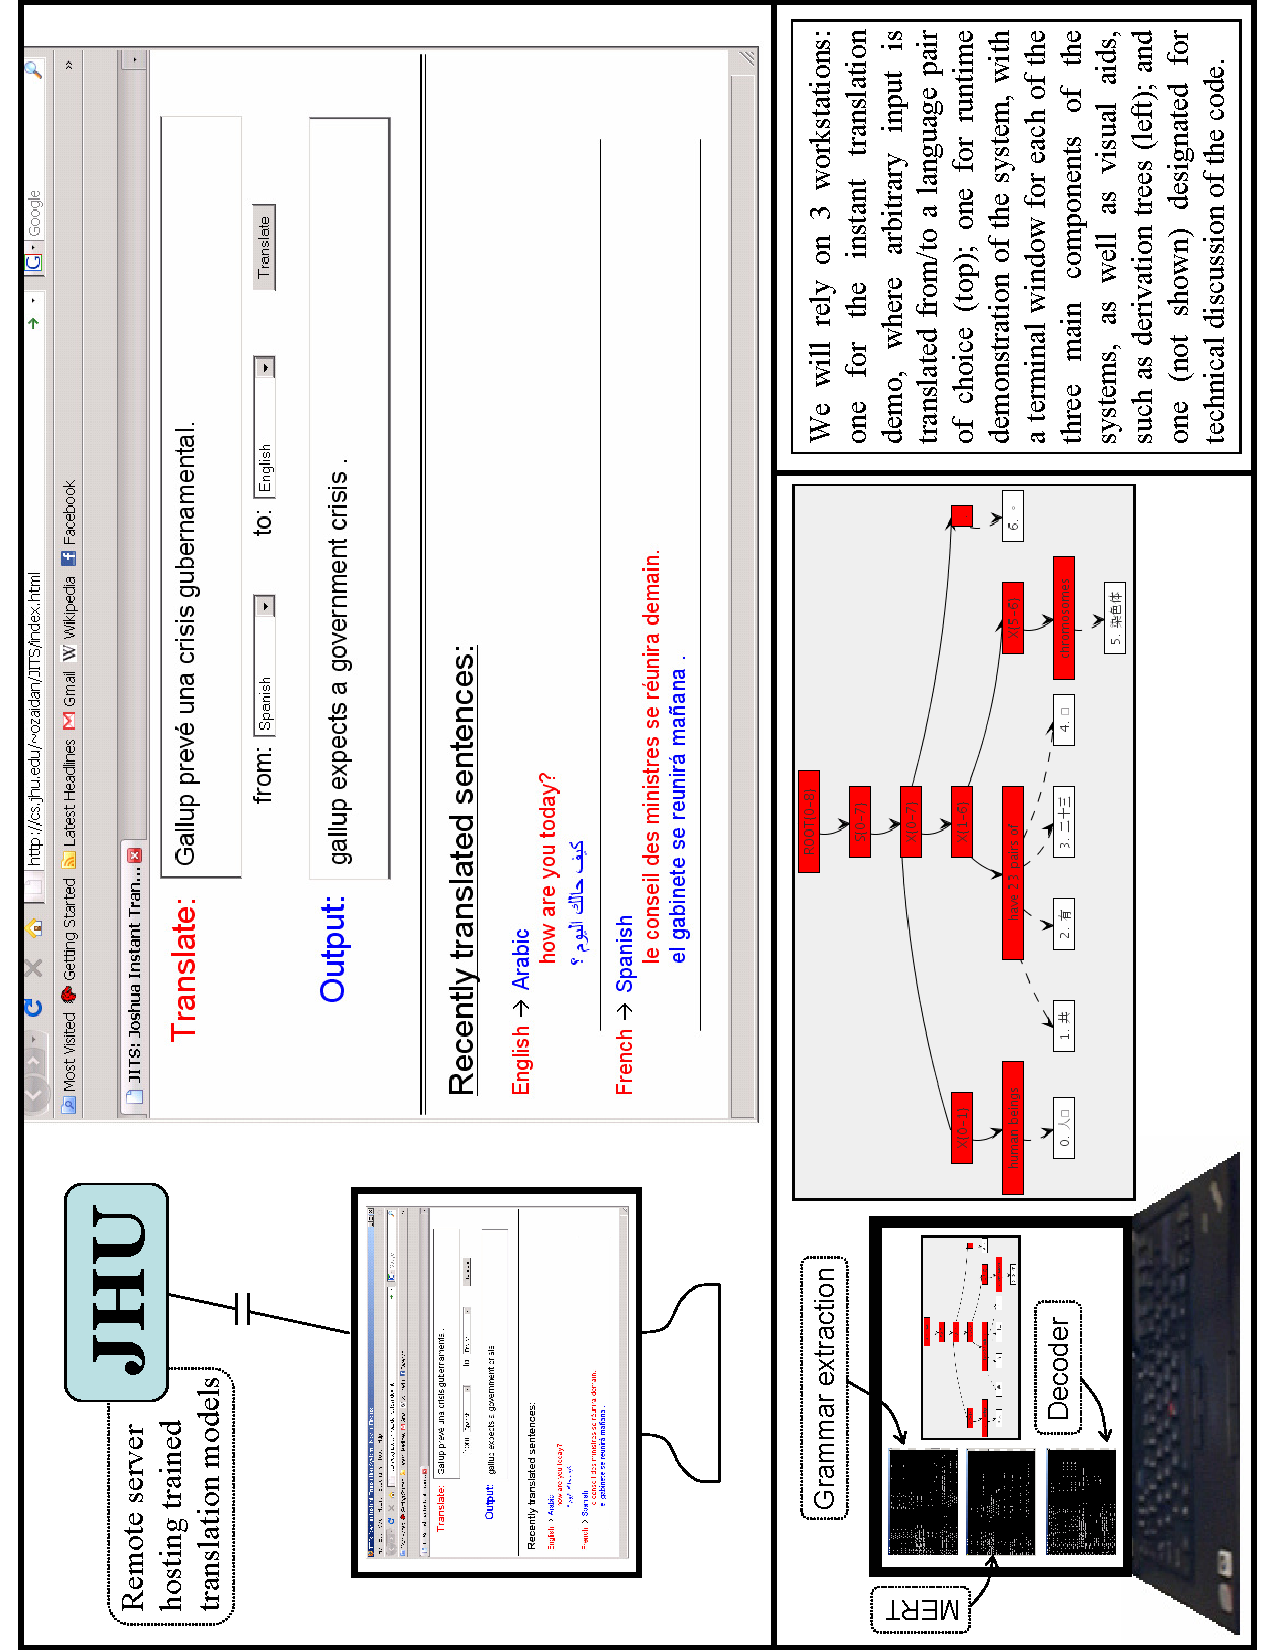
\includegraphics[scale=0.75]{demo-setup.pdf}
\caption{Proposed setup of our demonstration.}
\label{fig:setup}
\end{figure*}
\end{center}

%%%lzf add this section

%%%%%%%%%%%%%%%%%%%%%%%%%%%%%%%%%%%%%%%%%%%%%%%%%%%%%

%\section*{Acknowledgments}
%This research was supported in part by the Defense Advanced Research Projects Agency's GALE program under Contract No.\,HR0011-06-2-0001 and the National Science Foundation under grants No.\,0713448 and 0840112. The views and findings are the authors' alone.

%%%%%%%%%%%%%%%%%%%%%%%%%%%%%%%%%%%%%%%%%%%%%%%%%%%%%

\bibliographystyle{acl}
\bibliography{../bibliography}
\end{document}
